% Requires graphicx. Use figure* for full-width figures in a two-column article.
\begin{figure}[tbp]
\centering
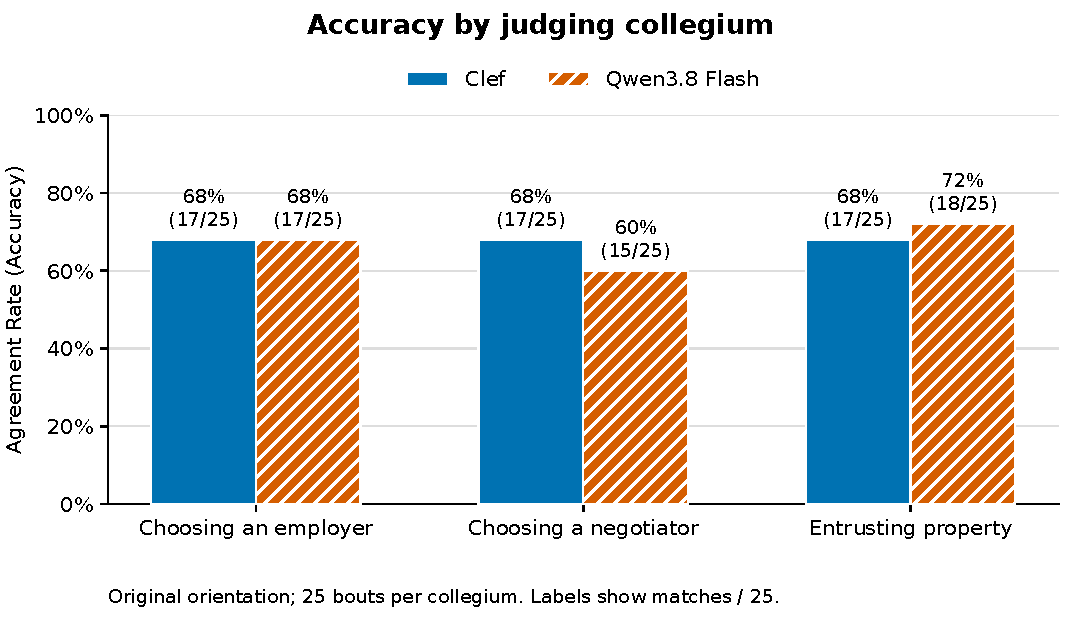
\includegraphics[width=\linewidth]{figures/figure1_accuracy_by_collegium.pdf}
\caption{Agreement Rate (Accuracy) by judging collegium in main run 015.
Each bar compares the model majority with the human majority in the original
orientation; labels give the percentage and number of matches out of 25 bouts.
The collegia select an employer, a negotiator, or a person to whom property
would be entrusted, respectively.}
\label{fig:accuracy-collegia}
\end{figure}

\begin{figure}[tbp]
\centering
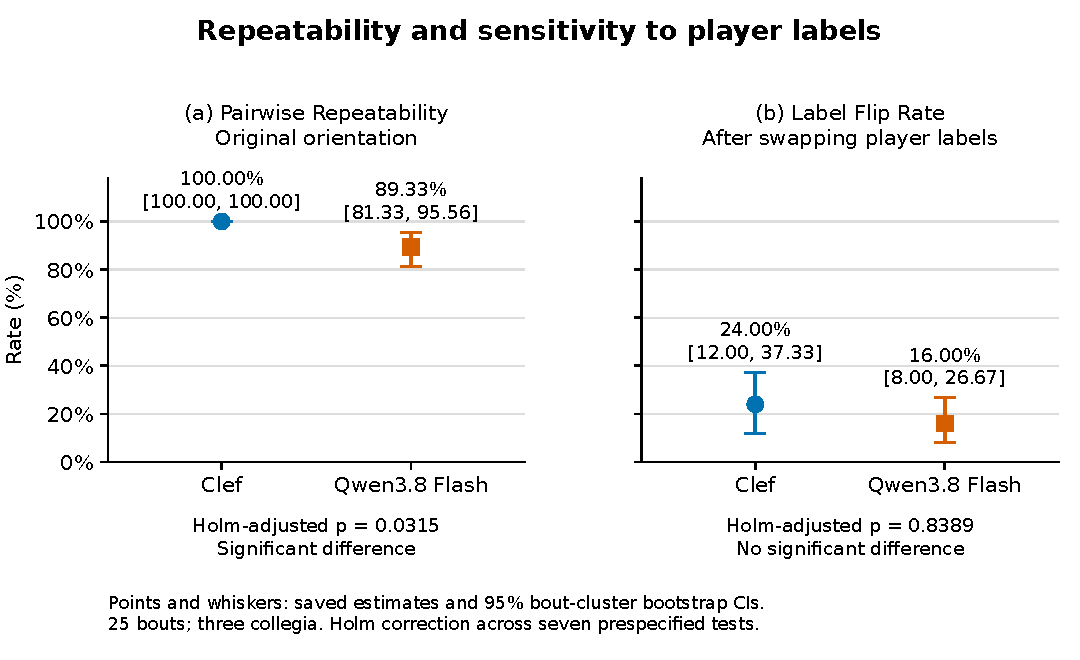
\includegraphics[width=\linewidth]{figures/figure2_repeatability_label_flip.pdf}
\caption{Repeatability and sensitivity to player-label swapping in main run 015.
(a) Pairwise Repeatability among three model votes per bout-collegium case in
the original orientation (higher indicates greater repeatability).
(b) Label Flip Rate after swapping labels and mapping decisions back to the
original participant identities (lower indicates greater invariance).
Points and whiskers show saved estimates and 95\% percentile bootstrap
intervals clustered by bout (25 bouts; three collegia).
Holm-adjusted permutation-test $p$-values assess each difference separately,
using the prespecified family of seven tests. The repeatability difference is
significant; the Label Flip Rate difference is not.
Clef's repeatability interval collapses at 100\% in the saved bootstrap sample;
this does not establish population certainty. Intervals based on 25 independent
bouts may be unstable.}
\label{fig:repeatability-label-flip}
\end{figure}
